
% File: basic_elements.tex
\documentclass{standalone}
\usepackage{pgfplots}
\pgfplotsset{compat=1.18}
\usepackage[american]{circuitikz}
\usepackage{cmbright}

\definecolor{myred}{RGB}{170,0,0}
\definecolor{myblue}{RGB}{0,0,220}

\ctikzset{bipoles/resistor/height=0.2}
\ctikzset{bipoles/resistor/width=0.5}


\begin{document}
% Simple RC circuit, with equations, and plots of different quantities.
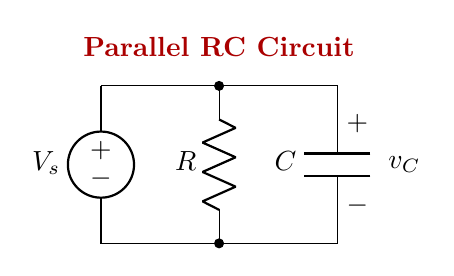
\begin{tikzpicture}
    % Subtitle for the circuit.
    \node[anchor=center, color=myred] at (1.5, 0.5) {\textbf{Parallel RC Circuit}};
    \begin{scope}
        \draw (0, 0)
            to[short, -*] ++(1.5, 0)
            to[R, l_={$R$}, -*] ++(0, -2)
            to[short] ++(-1.5, 0)
            to[V, l={$V_s$}, invert] ++(0, 2);
        \draw (1.5, 0)
            to[short] ++(1.5, 0)
            to[C, l_={$C$}, v^={$v_C$}] ++(0, -2)
            to[short] ++(-1.5, 0);
    \end{scope}
\end{tikzpicture}
\end{document}